\chapter{Theoretical background}
\lhead{Theoretical background}
\rhead{Radu-George Rusu}
\label{TheoreticalBackground}

This chapter will briefly describe the theoretical models used in the experiments presented in this paper.

\section{Expectation-Maximization}
The Expectation-Maximization (EM) is an algorithmic template for finding the Maximum Likelihood Estimation (MLE) parameters in statistical models which are based on missing or latent data.\\
The Maximum Likelihood Estimation problem can be defined as follows:

\fbox{
\begin{minipage}{\textwidth}
\textbf{MLE Problem}\\
\textbf{Input}\\
Y - set of observed data\\
$p$ - probability distribution that we assume generated the Y data set

\textbf{Output}\\
 $h^{MLE} = \underset{h}{argmax}$  $L(Y | h) = \underset{h}{argmax}$  $p(Y | h) $, where $h$ is the set of distribution parameters
\end{minipage}
}

 When the entire set Y is formed out of observable data, then the above problem can be easily solved. A common approach for this instance of the problem, is to take the derivative of the log-likelihood function and solve it for $h$. However, real life data is not always fully observed, and inside of the given data we have latent variables. In this particular case, the above-mentioned method doesn't work anymore, and an EM approach can be used.
 
 In the case of latent data we can consider the Y set as being a reunion between $X \cup Z = Y$, where X is the set of visible data, and Z is the set of hidden/latent data. The above-mentioned method doesn't work since it is impossible to compute $p(Z | h)$.
 
 \begin{figure}[H]
 	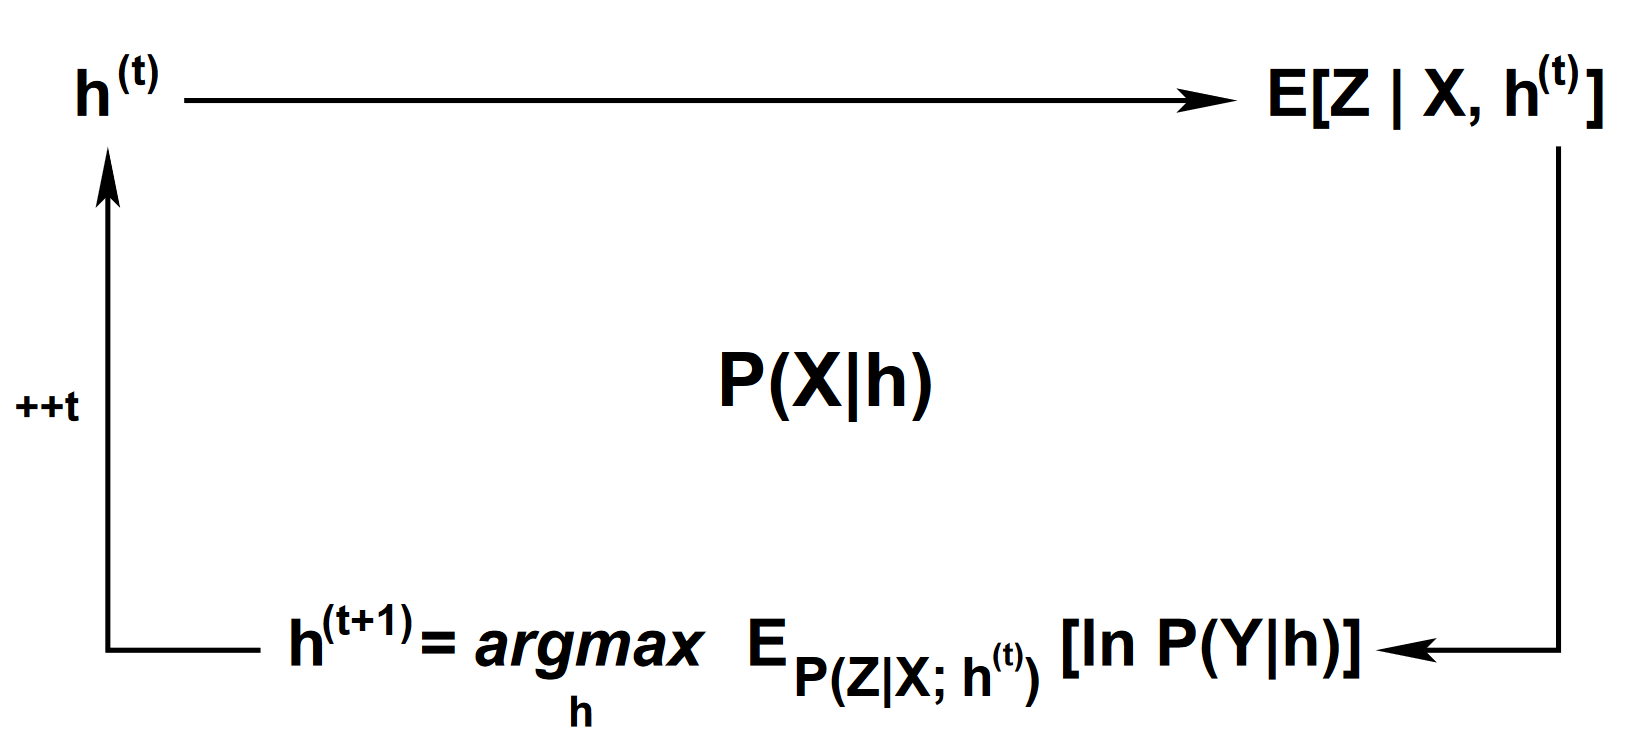
\includegraphics[width=\textwidth]{Pictures/004EMScheme.png}
 	\caption{EM Algorithm \cite{emCiortuz}}
 	\label{EmScheme}
 	%\textbf{Figure 2. Hill Climbing algorithm} [15]
 \end{figure}
 
 The EM algorithm (as show in \ref{EmScheme}) applies an iterative method, that for each iteration computes two steps:
 \begin{itemize}
 	\item E-Step: expectation of the latent variables, based on the distribution parameters from the previous iteration and the visible data ($\mathbf{E[Z | X, h^{(t)}]}$).
 	\item M-Step: based on the results from the E-Step, the latent variables, can be considered as observed and the $h$ parameters for this step can be solved like in the classic MLE problem.
 \end{itemize}

In the most basic form of this algorithm, the initial values for $h^{(0)}$ are randomly selected, and as a stop condition a maximum number of iterations can be used, but these two conditions can vary from problem to problem.
 
 
 

\section{Neural Networks for object detection}
In computer vision and object detection/recognition in images, the classical neural networks involved a high number of weights which have to be learned, which in turn, makes the networks work slow on images that are bigger in size and sometimes even impractical. The main advantage of the \textbf{Convolutional Neural Networks (CNN)} \cite{ConvNeuralNetwork} is the idea of using the convolution operator (\ref{Convolution}), which drastically reduces the number of weights to be learned and makes them usable in practice.

 \begin{figure}[H]
	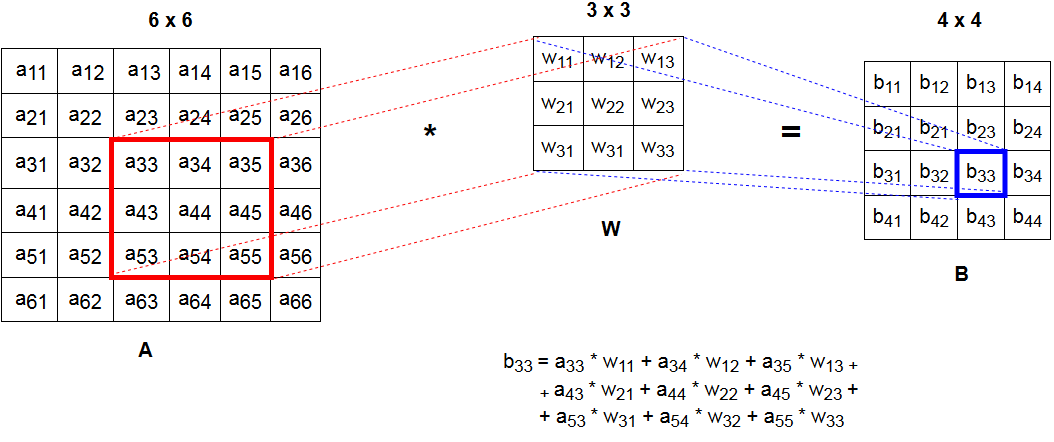
\includegraphics[width=\textwidth]{Pictures/006Convolution.png}
	\caption{Convolution operator \cite{ConvNeuralNetwork}}
	\label{Convolution}
	%\textbf{Figure 2. Hill Climbing algorithm} [15]
\end{figure}

Other two popular operators are the AveragePooling and MaxPooling, which as the name suggests, just extract either the average or the maximum value of the values in the corresponding square. Although these operators doesn't have as much expression power as the linear combination \ref{Convolution}, they don't have any weights to learn during the training phase.

The convolution operator result size depends on the following variables:
\begin{itemize}
	\item $n$ - size of the input image (considering the input image is squared)
	\item $f$ - size of the filter (also squared)
	\item $p$ - padding of the initial image
	\item $s$ - stride of the convolution operation
\end{itemize}
The convolution operator result size is:
$$ (n, n) * (f, f) = \bigg( \bigg\lfloor \frac{n + 2 \times p - f}{s} + 1 \bigg\rfloor , \bigg\lfloor \frac{n + 2 \times p - f}{s} + 1 \bigg\rfloor \bigg)$$

To observe the advantages of CNN over the classical NN we can take an example of a network formed only of two layers. A first one of size $1024\times1024$ which can be viewed as the input image, that is given in the grayscale, and a second layer of size $512\times512$, which is a first feature extraction layer of size $512\times512$.

In a classical neural network every input from the first layer must be connected with every output on the second layer, and every connection has it's own weight, which, in the above case, would result in computing $1024 \times 1024 \times 512 \times 512 = 274,877,906,944$ weights. Also, in computer vision problem there is a need of more than one intermediate layer to extract the features inside an image.

In the case of CNNs, the only weights that have to be computed for a layer are the values inside the filter, which in the above example can be considered a filter of size $512 \times 512 = 262,144‬$ with a stride of 1 and no padding. The number of weights that will be learned it's way less than in the case of classical neural networks, which allow more layers, and makes the CNN more practical for this problem. Also, in practical cases, the convolution operator can be an average/maximum over the target values, instead of a linear combination, and there will be no weights to learn on that level.

 \begin{figure}[H]
	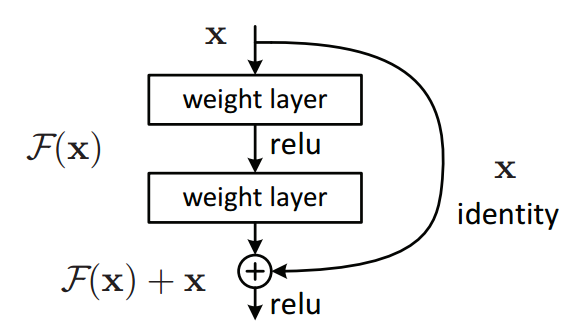
\includegraphics[width=\textwidth]{Pictures/007SkipConnection.png}
	\caption{Residual Block \cite{ResNetPaper}}
	\label{SkipConnection}
	%\textbf{Figure 2. Hill Climbing algorithm} [15]
\end{figure}

Another issue that occurs in practical object detection in image cases, is the depth of the network. In order to learn complex features inside an image, a neural network needs a high number of layers, to have space for learning every feature, which, in practice, leads to the vanishing gradient problem \cite{ResNetPaper}. This problem makes the training of these networks hard or even impossible, depending on the task. To solve this \textbf{Residual Networks} \cite{ResNetPaper} were developed.

The fundamental idea of these networks is the addition of the residual blocks (\ref{SkipConnection}). In this blocks, the inputs are once again added to the output value, before the activation function, avoiding a "squishing" derivative, which in turn will result in a higher overall derivative of the entire block.

With these methods, neural networks structures with 34, 50 or 152 layers were developed and used as show in \ref{ResNetExample}.

 \begin{figure}[H]
	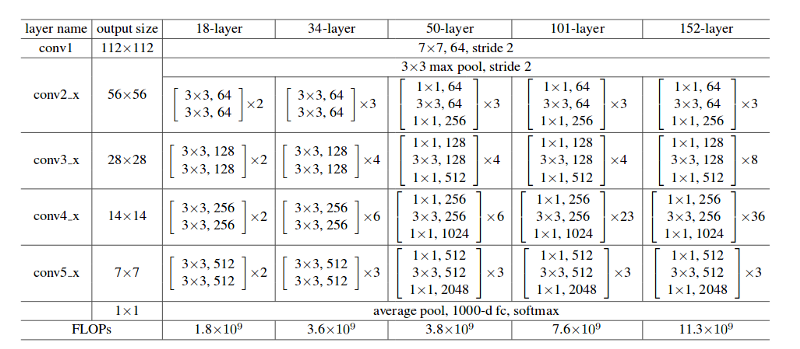
\includegraphics[width=\textwidth]{Pictures/008ResNetExample.png}
	\caption{Residual Networks Structure \cite{ResNetPaper}}
	\label{ResNetExample}
	%\textbf{Figure 2. Hill Climbing algorithm} [15]
\end{figure}

The neural networks described above behave well on object recognition and object detection problems. Another common case in image processing is the segmentation problem, where similar pixels inside a picture are grouped together. In this particular case, the CNN might not work well in the form described above, because every pixel of the image can have it's own classification, and the convolution operator is specialized in contracting image features, hence reducing the number of outputs of the network. To solve this problem, \textbf{U-Nets} networks \cite{Unet} have been developed. The name U-Net comes from the visual representation of the architecture (\ref{UnetArchitecture}) which resembles an U. There are two main parts of this architecture, the contracting path, and the expansive path. The contracting path behaves as an usual convolutional neural network extracting features from the image. The expansive path uses the Transposed Convolution Operator, which helps the networks reconstruct the image at the initial resolution, from the feature vector that was computed by the contracting path.

 \begin{figure}[H]
	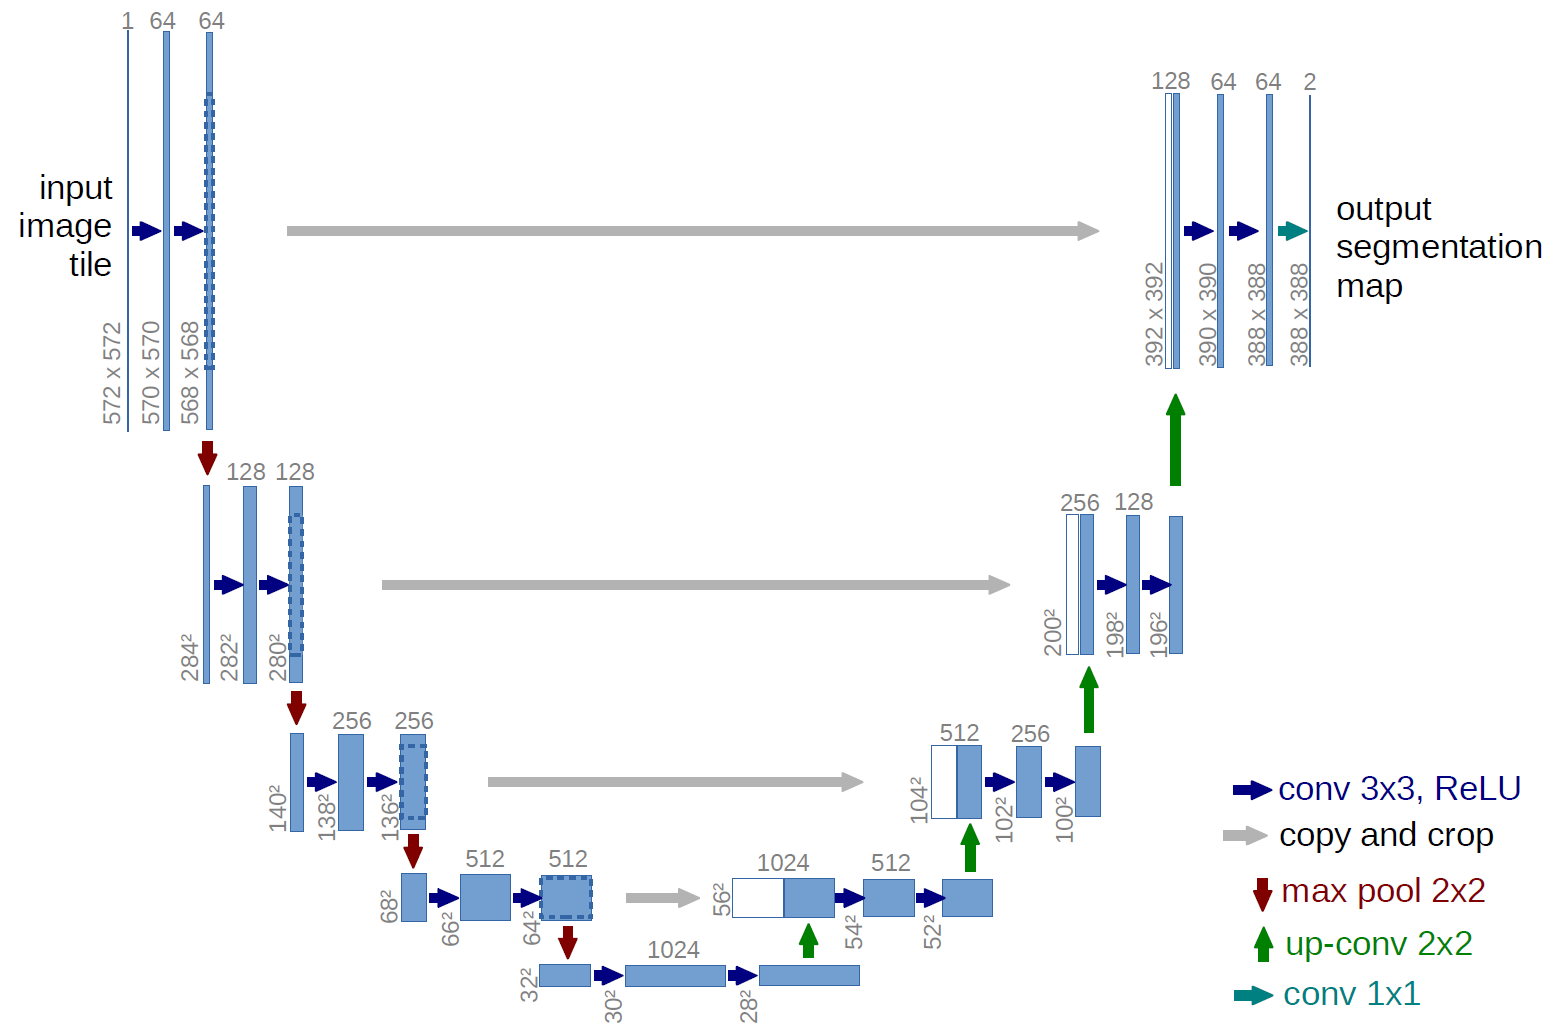
\includegraphics[width=\textwidth]{Pictures/012Unet.png}
	\caption{U-Net Architecture \cite{Unet}}
	\label{UnetArchitecture}
	%\textbf{Figure 2. Hill Climbing algorithm} [15]
\end{figure}